\documentclass[10pt]{article}
\usepackage{graphicx}
\usepackage[backend=biber,style=numeric,sorting=ynt]{biblatex}

\addbibresource{references.bib}


%This document is intended to be a template for your reports and should be used as a starting point. You should remove the instructions and replace them with your own text.

\title{Optical Activity} % Write the name of the experiment here
\author{Rahmanyaz Annyyev, Hikmat Gulaliyev} % Members of the lab group
 
\date{28 March 2024} % Date of the report

% This semester you will be using LaTeX to write your lab reports. It is a typesetting system that allows you to write your report in a text editor and then typeset it into a professional looking document. It is a very powerful tool that is used by many scientists and engineers. It is also a very useful skill to have. It may seem daunting at first sight, but it is actually very easy to learn.  It has many documents and tutorials online, and you can also ask the TA's for help. 

% The best place to start is overleaf.com. It is a web based LaTeX editor that allows you to write your report in a web browser. It also has a built in compiler that will typeset your document into a PDF. In order to start using overleaf, you need to create an account, create project and upload the report template to overleaf. Once you do that, you are good to go. You can also download the LaTeX editor of your choice and use that to write your report.


\begin{document}
\maketitle

\begin{abstract}
The abstract is a short summary of the report. It consicely describes the experiment and the results. A reader should be able to understand the main questions that are being investigated, the methods used to answer the questions, and results of the investigation from the abstract. Ideally, it should be between 100-200 words.

\end{abstract}

\section{Introduction}

In the introduction you should give a brief overview of the experiment. You should start with a brief description of the theoretical background behind the experiment. You should also mention the methods used in the experiment. You are expected to cite your sources\cite{Bravyi_2020} midtext.\footnote{More information on how to do this can be found in the references section.}

%You can use the '\footnote' command to add a footnote to your document.

You can insert an inline equation using the \$ sign. As in $E=mc^2$. To display an equation in the middle of the page use the following:

\begin{equation}
    \int \frac{1}{x} dx = \ln|x| + C
\end{equation}

\section{Data \& Results}

\begin{table}[ht]
    \centering
    \begin{tabular}{|c|c|c|c|}
        \hline
        Something & Something & Something & Something \\
        \hline
        1234 & 1234 & 1234 & 1234 \\
        \hline
    \end{tabular}
    \caption{This is a caption for the table.}
    \label{tab:ex}
\end{table}

\begin{figure}[ht]
    \centering
    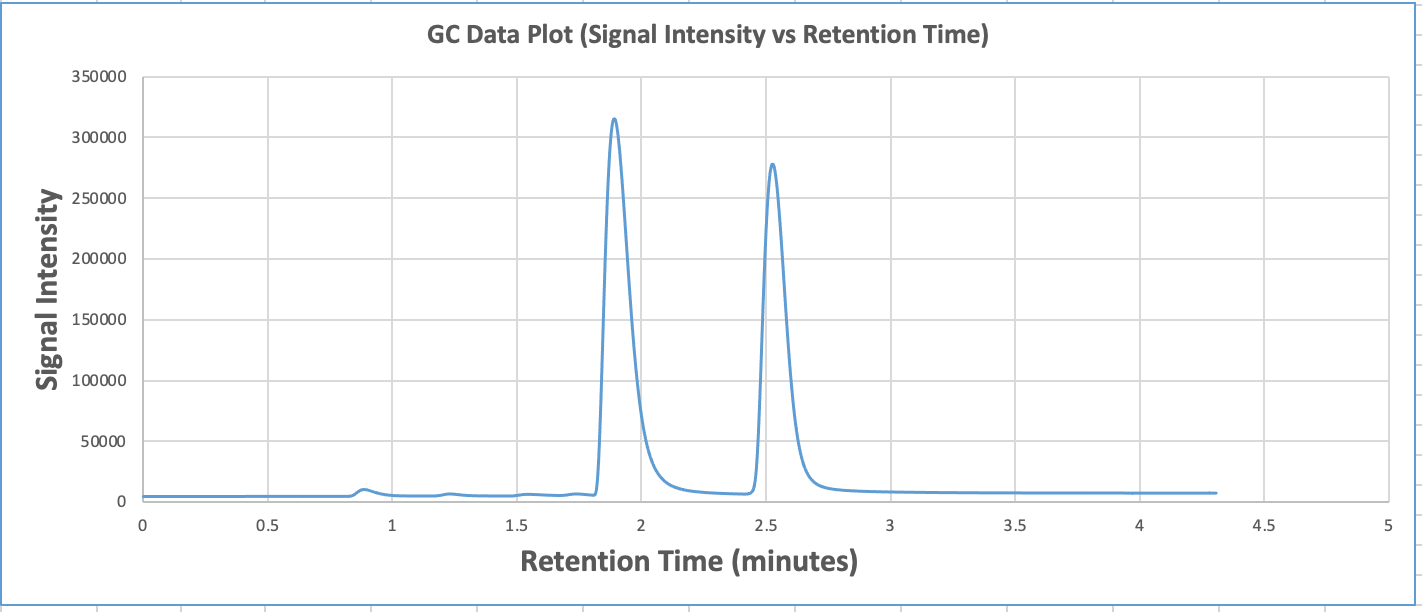
\includegraphics[width=0.72\textwidth]{example_figure.png}
    \caption{This is a caption for the figure.}
    \label{fig:ex}
\end{figure}

In this section, you are to present the data you obtain from the experiment,which is mostly going to be presented in the form of a table as in Table \ref{tab:ex} or in the form of a graph as in Figure \ref{fig:ex}. The manuals for the experiments have instructions on how to present the data, and in the case of any ambiguity you TA will provide you with the necessary information. You should also include any calculations you do in this section. A brief discussion of the results should also be included.

\section{Discussion \& Conclusion}

In this section, you are expected to discuss the limitations of the experiment and how these limitations may have affected the results. Meaning, you are to discuss the possible errors, the approximations you made in obtaining physical data, and the discrepancies you see between the results you obtain and the theoretical values or the values reported in the literature. You should also discuss the possible improvements that can be made to the experiment. 

\printbibliography

% You should put your references in the references.bib file. You can use an  online bibtex generator to generate the bibtex entry for your reference. You can cite your references in the text using the \cite{reference_title} command. The '\printbibliography' command will print the bibliography at the end of the document. 

\end{document}